\documentclass{article}
\usepackage[T1]{fontenc}
\usepackage{lmodern}
\usepackage{graphicx}
\usepackage{amsmath,amssymb}
\usepackage[a4paper,margin=2cm]{geometry}
\usepackage[absolute,overlay]{textpos}
\setlength{\TPHorizModule}{1mm}
\setlength{\TPVertModule}{1mm}
\usepackage[indonesian]{babel}
\usepackage{hyperref}
\setlength{\emergencystretch}{2em}
% unit: Halaman 15

\begin{document}

% === Halaman 15 (llm) ===

Matriks PC-2 berikut:

\vspace{20mm}

Jadi, $K_i$ merupakan penggabungan bit-bit $C_i$ pada posisi:
\[ 14, 17, 11, 24, 1, 5, 3, 28, 15, 6, 21, 10 \\
 23, 19, 12, 4, 26, 8, 16, 7, 27, 20, 13, 2 \]

dengan bit-bit $D_i$ pada posisi:
\[ 41, 52, 31, 37, 47, 55, 30, 40, 51, 45, 33, 48 \\
 44, 49, 39, 56, 34, 53, 46, 42, 50, 36, 29, 32 \]

Setiap kunci internal $K_i$ mempunyai panjang 48 bit.

% deskripsi: Tabel matriks permutasi PC-2 yang berisi angka-angka posisi bit.
% bbox normalisasi: [0.0330, 0.1350, 0.5910, 0.3250]
\begin{textblock*}{117.18mm}(6.93mm,40.10mm)
\noindent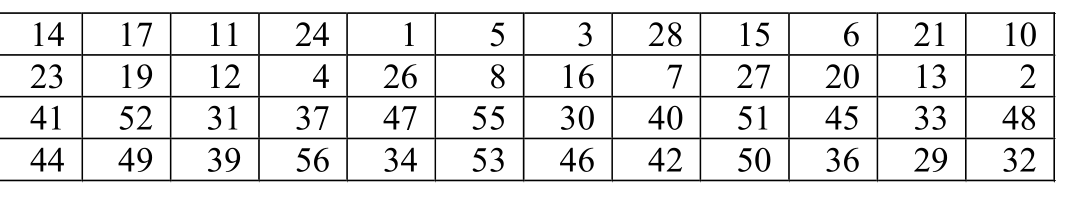
\includegraphics[width=117.18mm,height=56.43mm]{../../images/llm/page_015_img_01.png}%
\end{textblock*}

% deskripsi: Diagram alir proses pembangkitan kunci internal Ki menggunakan permutasi PC-1, operasi Left Shift pada register C dan D, serta permutasi PC-2.
% bbox normalisasi: [0.6550, 0.1350, 0.9600, 0.8450]
\begin{textblock*}{64.05mm}(137.55mm,40.10mm)
\noindent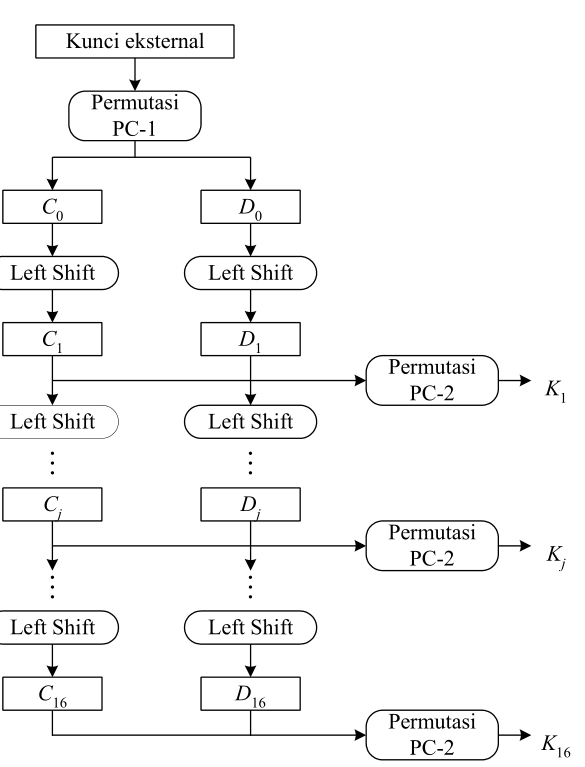
\includegraphics[width=64.05mm,height=210.87mm]{../../images/llm/page_015_img_02.png}%
\end{textblock*}

\end{document}
